\documentclass[a4paper,12pt]{extarticle}
\usepackage[utf8x]{inputenc}
\usepackage[T1,T2A]{fontenc}
\usepackage[russian]{babel}
\usepackage{hyperref}
\usepackage{indentfirst}
\usepackage{listings}
\usepackage{color}
\usepackage{xcolor}
\usepackage{here}
\usepackage{array}
\usepackage{multirow}
\usepackage{graphicx}
\usepackage{amsmath}

\hypersetup{
    colorlinks = false,
    linkbordercolor = {white}
}

\definecolor{string}{HTML}{B40000} % цвет строк в коде
\definecolor{comment}{HTML}{008000} % цвет комментариев в коде
\definecolor{keyword}{HTML}{1A00FF} % цвет ключевых слов в коде
\definecolor{morecomment}{HTML}{8000FF} % цвет include и других элементов в коде
\definecolor{сaptiontext}{HTML}{FFFFFF} % цвет текста заголовка в коде
\definecolor{сaptionbk}{HTML}{999999} % цвет фона заголовка в коде
\definecolor{bk}{HTML}{FFFFFF} % цвет фона в коде
\definecolor{frame}{HTML}{999999} % цвет рамки в коде
\definecolor{brackets}{HTML}{B40000} % цвет скобок в коде

\usepackage{caption}
\renewcommand{\lstlistingname}{Программа} % заголовок листингов кода

\bibliographystyle{ugost2008ls}

\usepackage{listings}
\lstset{ %
	extendedchars=\true,
	keepspaces=true,
	language=Python,						% choose the language of the code
	% Цвета
	keywordstyle=\color{keyword}\ttfamily\bfseries,
	%stringstyle=\color{string}\ttfamily,
	stringstyle=\ttfamily\color{red!50!brown},
	commentstyle=\color{comment}\ttfamily\itshape,
	morecomment=[l][\color{morecomment}]{\#},
	basicstyle=\footnotesize,		% the size of the fonts that are used for the code
	numbers=left,					% where to put the line-numbers
	numberstyle=\footnotesize,		% the size of the fonts that are used for the line-numbers
	stepnumber=1,					% the step between two line-numbers. If it is 1 each line will be numbered
	numbersep=5pt,					% how far the line-numbers are from the code
	backgroundcolor=\color{white},	% choose the background color. You must add \usepackage{color}
	showspaces=false				% show spaces adding particular underscores
	keywordstyle=color{blue}\bfseries, 
	showstringspaces=false,			% underline spaces within strings
	showtabs=false,					% show tabs within strings adding particular underscores
	frame=single,          		% adds a frame around the code
	tabsize=2,						% sets default tabsize to 2 spaces
	captionpos=t,					% sets the caption-position to top
	breaklines=true,				% sets automatic line breaking
	breakatwhitespace=false,		% sets if automatic breaks should only happen at whitespace
	escapeinside={\%*}{*)},			% if you want to add a comment within your code
	postbreak=\raisebox{0ex}[0ex][0ex]{\ensuremath{\color{red}\hookrightarrow\space}},
	texcl=true,
	inputpath=listings,                     % директория с листингами
}

\usepackage[left=2cm,right=2cm,
top=2cm,bottom=2cm,bindingoffset=0cm]{geometry}

%% Нумерация картинок по секциям
\usepackage{chngcntr}
\counterwithin{figure}{section}
\counterwithin{table}{section}

%%Точки нумерации заголовков
\usepackage{titlesec}
\titlelabel{\thetitle.\quad}
\usepackage[dotinlabels]{titletoc}

%% Оформления подписи рисунка
\addto\captionsrussian{\renewcommand{\figurename}{Рисунок}}
\captionsetup[figure]{labelsep = period}

%% Подпись таблицы
\DeclareCaptionFormat{hfillstart}{\hfill#1#2#3\par}
\captionsetup[table]{format=hfillstart,labelsep=newline,justification=centering,skip=-10pt,textfont=bf}

%% Путь к каталогу с рисунками
\graphicspath{{fig/}}

\begin{document}	% начало документа

% Титульная страница
%\begin{titlepage}	% начало титульной страницы

	\begin{center}		% выравнивание по центру

		Санкт-Петербургский Национально Исследовательский Университет\\
		информационных технологий, механики и оптики \\
		Кафедра систем управления и информатики\\[3cm]
		% название института, затем отступ 6см
		
		\huge \textbf{РЕФЕРАТ}\\[0.5cm]
		\large Электромеханические системы\\[0.1cm]
		\large Система автоматического управления квадракоптера Parrot ARDrone 2.0\\[2cm]

	\end{center}


	\begin{flushright} % выравнивание по правому краю
%		\begin{minipage}{0.5\textwidth} % врезка в половину ширины текста
%			\begin{flushleft} % выровнять её содержимое по левому краю

				\large Выполнили студенты группы P3335\\
				\large А.М. Зенкин\\[0.5cm]
				\large К.В. Карпов\\[0.5cm]
				
				\large Принял  к.т.н., доцент кафедры СУиР\\
				\sign[4cm]\large  М.С. Чежин\\
				\large Оценка: \sign\\
				«\underline{\hspace{0.7cm}}» \underline{\hspace{2cm}} \the\year г.

%			\end{flushleft}
%		\end{minipage}
	\end{flushright}
	
	\vfill % заполнить всё доступное ниже пространство

	\begin{center}
	\large Санкт-Петербург\\
	\large \the\year % вывести дату
	\end{center} % закончить выравнивание по центру

\thispagestyle{empty} % не нумеровать страницу
%\end{titlepage} % конец титульной страницы
\newpage


% Содержание
% Содержание
\renewcommand\contentsname{\centerline{Содержание}}
\tableofcontents
\thispagestyle{fancy}
\newpage




\section{Цель работы}
Написания программы для парсинга сайта с целью получения нужных данных, используюя Python. После загрузка полученной информации в Google Doc.

\section{Ход работы}

\subsection{Выбор среды программирования}
В качесте среды разработки был выбран PyCharm( рис. \ref{pic:pic_1}), разработанный копанией JetBrains на основе IntelliJ IDEA. Данная среда имеет множество достоинств, некоторые из их приведены ниже:

\begin{itemize}
	\item    Статический анализ кода, подсветка синтаксиса и ошибок.
	\item    Навигация по проекту и исходному коду: отображение файловой структуры проекта, быстрый переход между файлами, классами, методами и использованиями методов.
	\item    Рефакторинг: переименование, извлечение метода, введение переменной, введение константы, подъём и спуск метода и т. д.
	\item    Встроенный отладчик для Python
	\item    Поддержка систем контроля версий: общий пользовательский интерфейс для Mercurial, Git, Subversion, Perforce и CVS с поддержкой списков изменений и слияния
\end{itemize}
	
\begin{figure}[H]
	\begin{center}
		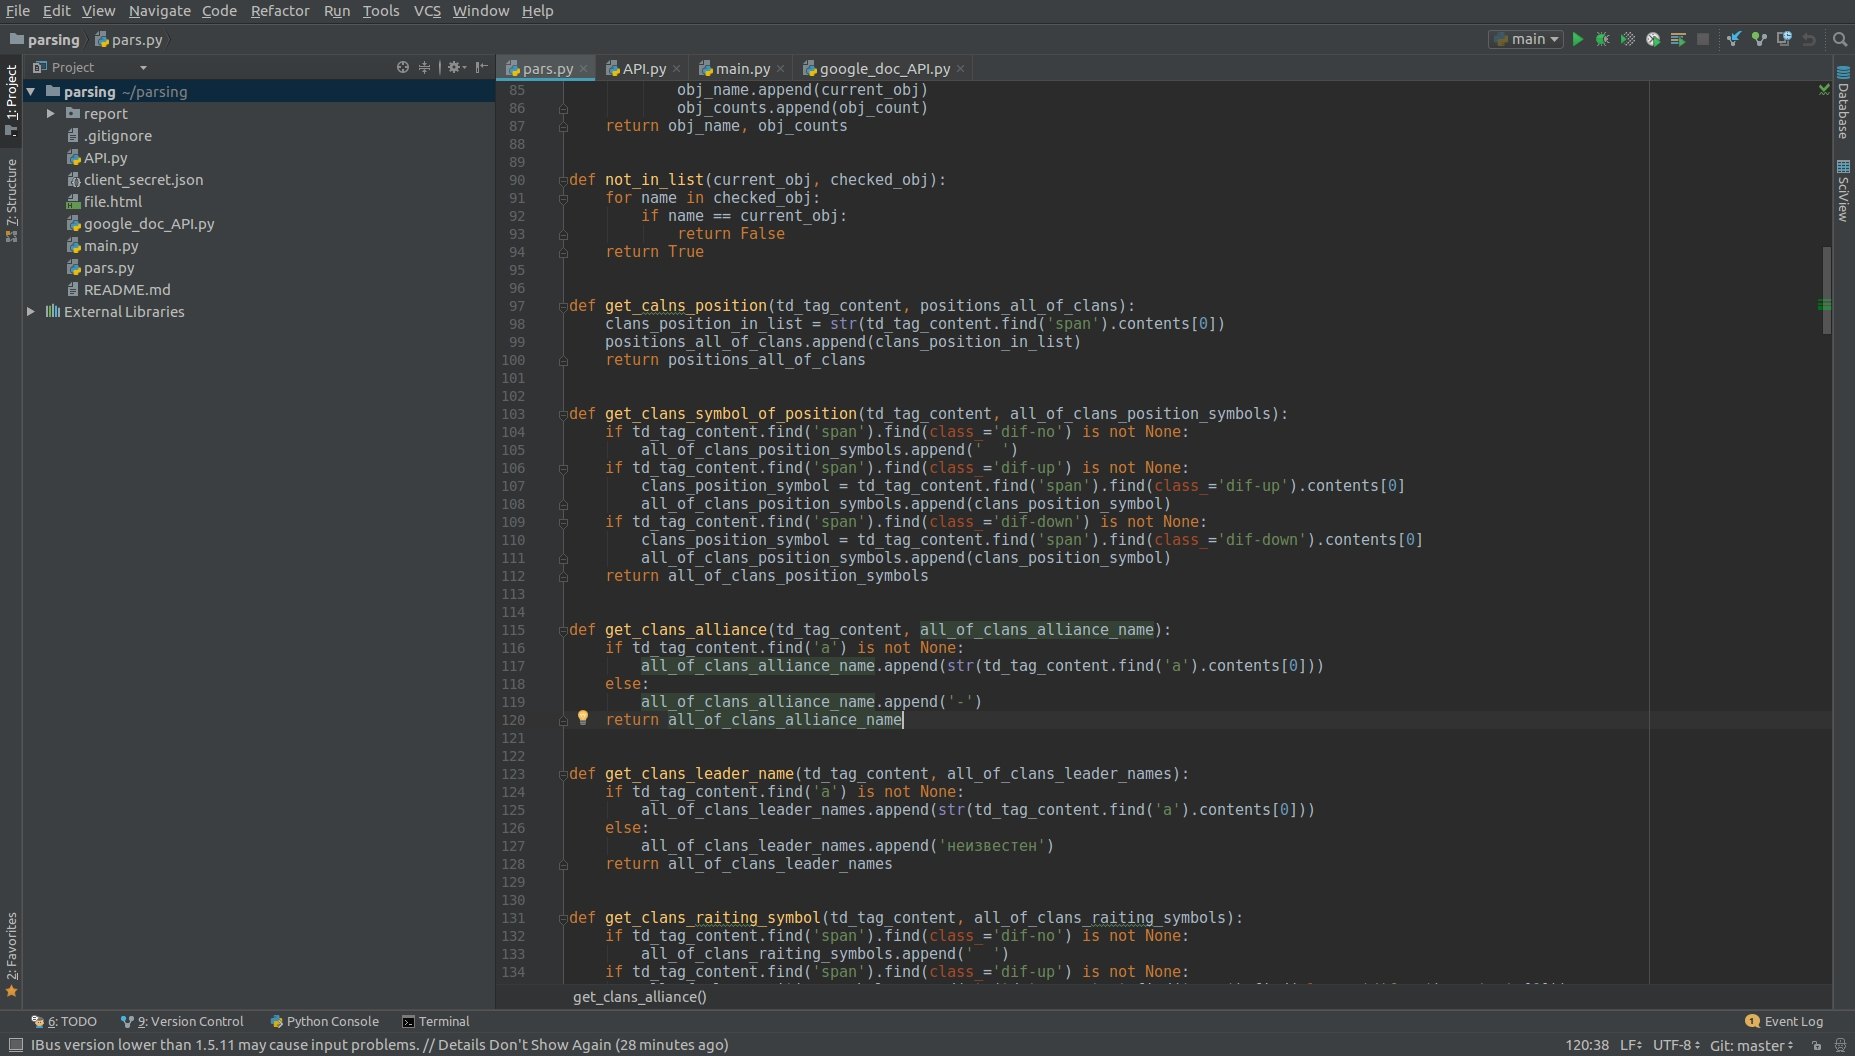
\includegraphics[scale=0.25]{PyCharm_2}
		\caption{- интерфейс PyCharm} 
		\label{pic:pic_1} % название для ссылок внутри кода
	\end{center}
\end{figure}

\subsection{Разбитие проекта на модули}
В ходе выполнения проекта было принято решение разбить его на следующие пакеты:

\begin{itemize}

	\item main.py
	\item pars.py
	\item API.py
	\item GoogleDocAPI.py
	
\end{itemize}

В модуле main содержится основная программа, которая вызывает все функции из модулей.

Модуль pars содержит функции для парсинга сайта и получения информации с него.

Модуль API позволяет пользователю общаться с программой и выводить информацию в коммандную строку.

Модуль GoogleDocAPI осуществляет работу с Google Doc.

\subsection{Описание модуля pars}

\subsubsection{get\_top\_50}
Возвращает всю информацию о топ 50 кланах.
\lstinputlisting[
	label=code:plot,
	caption={get\_top\_50},
]{Get_top_50.py}
\parindent=1cm

\newpage

\subsubsection{get\_clans\_position,  get\_clans\_symbol\_of\_position,\\ get\_clans\_alliance,  get\_clans\_leader\_name,\\  get\_clans\_rating\_symbol}
Вспомогательные функции для get\_top\_50. Возвращают позицию клана, маркер позиции, альянс клана, имя лидера клана и маркер рейтинга клана
\lstinputlisting[
	label=code:plot,
	caption={group of functions for get\_top\_50},
]{top_50.py}
\parindent=1cm

\newpage

\subsubsection{get\_clan\_info}
Основная функция, которая возвращеат всю информацию о выбранном клане.
\lstinputlisting[
	label=code:plot,
	caption={get\_clan\_info},
]{get_clan_info.py}
\parindent=1cm

\subsubsection{get\_header\_info}
Вспомогательная функция для get\_clan\_info. Возвращает данные о ссылке, лидере, персонажах, профессий, текучке, альянсе, холле, замке, крепости, "О клане" выбранного клана.
\lstinputlisting[
	label=code:plot,
	caption={get\_header\_info},
]{GetHeaderInfo.py}
\parindent=1cm

\subsubsection{get\_member\_table}
Вспомогательная функция для get\_clan\_info. Возвращает всю информацию о членах выбранного клана.
\lstinputlisting[
	label=code:plot,
	caption={get\_member\_table},
]{GetMemberTable.py}
\parindent=1cm

\subsubsection{get\_clans\_statistic}
Возвращает статистику по клану.
\lstinputlisting[
	label=code:plot,
	caption={get\_clans\_statistic},
]{GetClanStats.py}
\parindent=1cm

\newpage

\subsubsection{get\_server\_stats}
Возвращает статистику по серверу.
\lstinputlisting[
	label=code:plot,
	caption={get\_server\_stats},
]{GetServerStats.py}
\parindent=1cm

\subsubsection{get\_clan\_stats}
Возвращает статистику по клану.
\lstinputlisting[
	label=code:plot,
	caption={get\_clan\_stats},
]{GetClanStats.py}
\parindent=1cm

\newpage

\subsubsection{get\_profession\_stats}
Возвращает статистику по профессиям сервера.
\lstinputlisting[
	label=code:plot,
	caption={get\_profession\_stats},
]{GetProfStats.py}
\parindent=1cm

\subsubsection{get\_second\_profession}
Вспомогательная функция для GetProfessionStats.
\lstinputlisting[
	label=code:plot,
	caption={get\_second\_profession},
]{GetSecondProfession.py}
\parindent=1cm

\newpage

\subsubsection{calc\_persentage}
Возвращает проценты по количеству профессий.
\lstinputlisting[
	label=code:plot,
	caption={calc\_persentage},
]{CalcPersentage.py}
\parindent=1cm

\subsubsection{get\_html\_code,\\ get\_url\_from\_str, get\_id, is\_in\_html\_code,\\ get\_name\_of\_th, get\_obj\_info}
Вспомогательные функции.
\lstinputlisting[
	label=code:plot,
	caption={get\_html\_code},
]{GetHtmlCode.py}
\parindent=1cm

\lstinputlisting[
	label=code:plot,
	caption={get\_url\_from\_str},
]{GetUrlFromStr.py}
\parindent=1cm

\lstinputlisting[
	label=code:plot,
	caption={get\_id},
]{GetId.py}
\parindent=1cm

\lstinputlisting[
	label=code:plot,
	caption={is\_in\_html\_code},
]{IsInHtmlCode.py}
\parindent=1cm

\newpage

\lstinputlisting[
	label=code:plot,
	caption={get\_name\_of\_th},
]{GetNameOfTh.py}
\parindent=1cm

\lstinputlisting[
	label=code:plot,
	caption={get\_obj\_info},
]{GetObfInfo.py}
\parindent=1cm

\lstinputlisting[
	label=code:plot,
	caption={is\_title},
]{is_title.py}
\parindent=1cm

\lstinputlisting[
	label=code:plot,
	caption={not\_in\_list},
]{not_in_list.py}
\parindent=1cm

\newpage

\subsection{Описание модуля API}

\subsubsection{clear\_screen}
Очищает экран командной строки.
\lstinputlisting[
	label=code:plot,
	caption={clear\_screen},
]{clear_screen.py}
\parindent=1cm

\subsubsection{get\_full\_url}
Возвращает полный путь к странице.
\lstinputlisting[
	label=code:plot,
	caption={get\_full\_url},
]{get_full_url.py}
\parindent=1cm

\subsubsection{get\_server\_number}
Позволяет пользователю выбрать желаемый сервер.
\lstinputlisting[
	label=code:plot,
	caption={get\_server\_number},
]{get_server_number.py}
\parindent=1cm

\subsubsection{choose\_clan}
Позволяет пользователю выбрать желаемый клан.
\lstinputlisting[
	label=code:plot,
	caption={choose\_clan},
]{choose_clan.py}
\parindent=1cm

\subsubsection{print\_top\_50}
Выводит в командную строку топ 50 кланов.
\lstinputlisting[
	label=code:plot,
	caption={print\_top\_50},
]{print_top_50.py}
\parindent=1cm

\subsubsection{print\_clan\_information}
Выводит в командную строку информацию о выбранном клане.
\lstinputlisting[
	label=code:plot,
	caption={print\_clan\_information},
]{print_clan_information.py}
\parindent=1cm

\newpage

\subsubsection{print\_clan\_stats}
Выводит в командную строку статистику клана.
\lstinputlisting[
	label=code:plot,
	caption={print\_clan\_stats},
]{print_clan_stats.py}
\parindent=1cm

\subsubsection{print\_server\_stats}
Выводит в командную строку статистику по серверу.
\lstinputlisting[
	label=code:plot,
	caption={print\_server\_stats},
]{print_server_stats.py}
\parindent=1cm

\newpage

\subsubsection{print\_server\_pofession\_stats}
Выводит в командную строку статистику по профессиям сервера.
\lstinputlisting[
	label=code:plot,
	caption={print\_server\_pofession\_stats},
]{print_server_pofession_stats.py}
\parindent=1cm

\newpage

\subsection{Описание модуля GoogleDocAPI}

\subsubsection{add\_to\_google\_sheet}
Добавляет данный в Google Doc.
\lstinputlisting[
	label=code:plot,
	caption={add\_to\_google\_sheet},
]{add_to_google_sheet.py}
\parindent=1cm

\subsubsection{add\_prof\_server\_stats}
Добавляет статистику по профессиям сервера в Google Doc.
\lstinputlisting[
	label=code:plot,
	caption={add\_prof\_server\_stats},
]{add_prof_server_stats.py}
\parindent=1cm

\subsubsection{load\_all\_data\_in\_google\_doc}
Загружает все в Google Doc.
\lstinputlisting[
	label=code:plot,
	caption={load\_all\_data\_in\_google\_doc},
]{load_all_data_in_google_doc.py}
\parindent=1cm

\newpage

\subsection{Описание main}

\lstinputlisting[
	label=code:plot,
	caption={main},
]{main.py}
\parindent=1cm

\newpage

\subsection{Примеры работы программы}

Примеры работы программы приведены на рисунках \ref{pic:pic_2} - \ref{pic:pic_11}.

\begin{figure}[H]
	\begin{center}
		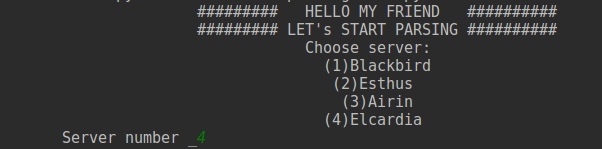
\includegraphics[scale=0.5]{1}
		\caption{- выбор сервера} 
		\label{pic:pic_2} % название для ссылок внутри кода
	\end{center}
\end{figure}

\begin{figure}[H]
	\begin{center}
		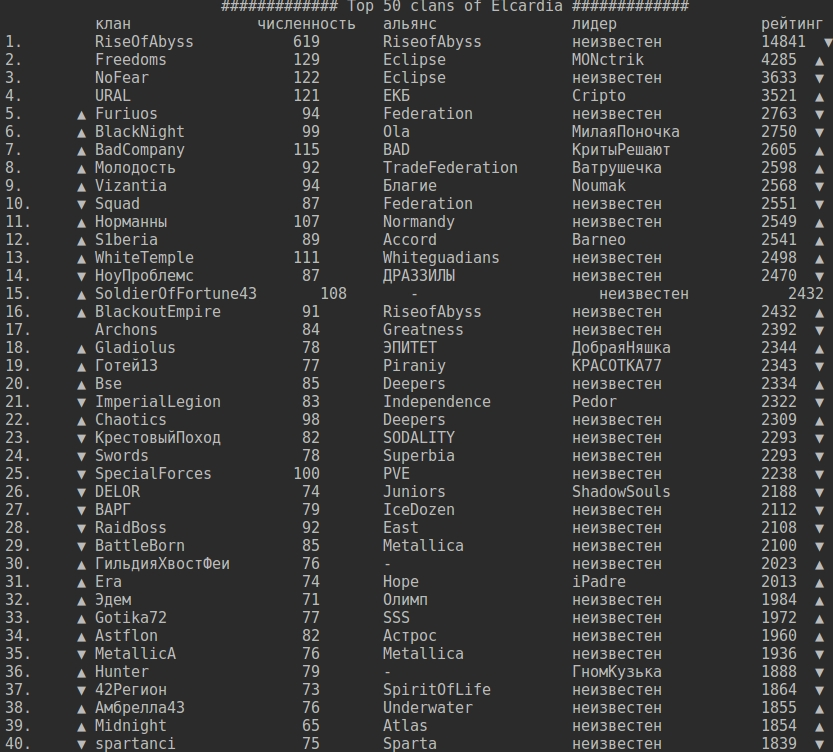
\includegraphics[scale=0.5]{2}
		\caption{- топ 50 кланов} 
		\label{pic:pic_3} % название для ссылок внутри кода
	\end{center}
\end{figure}

\begin{figure}[H]
	\begin{center}
		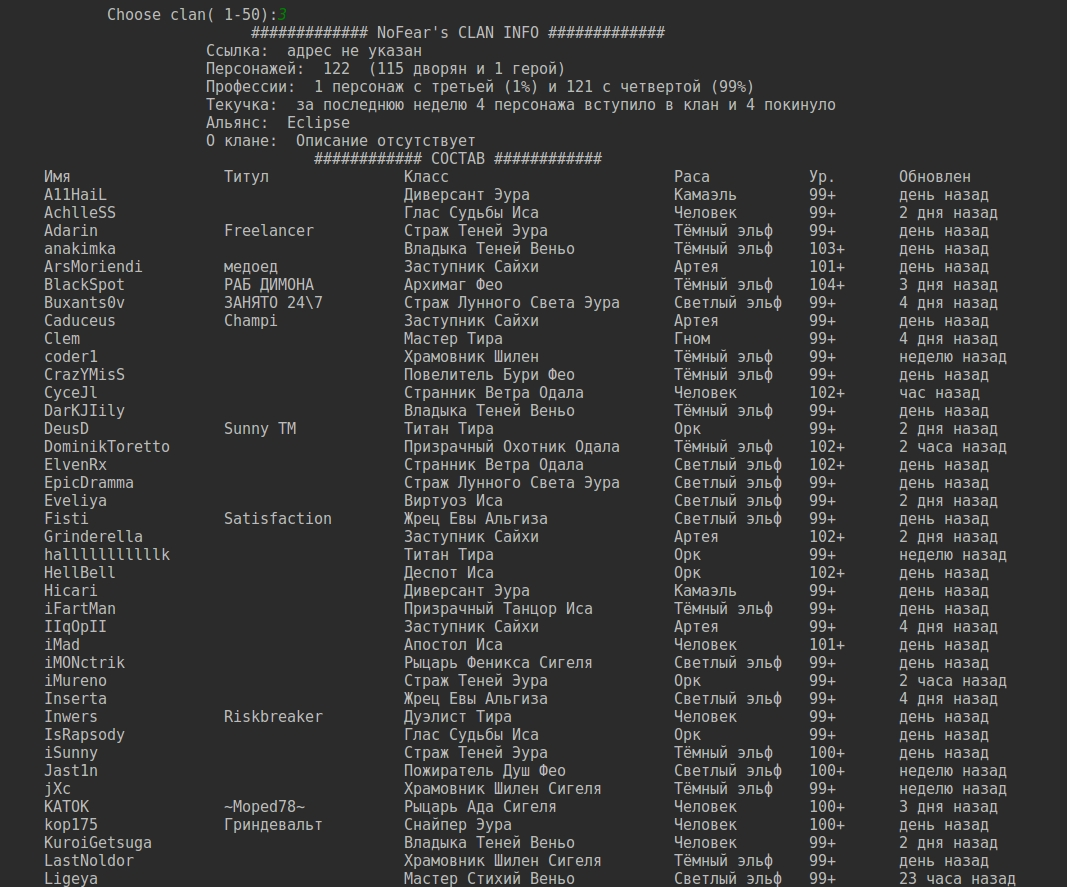
\includegraphics[scale=0.4]{3}
		\caption{- информация о выбранном клане} 
		\label{pic:pic_4} % название для ссылок внутри кода
	\end{center}
\end{figure}

\begin{figure}[H]
	\begin{center}
		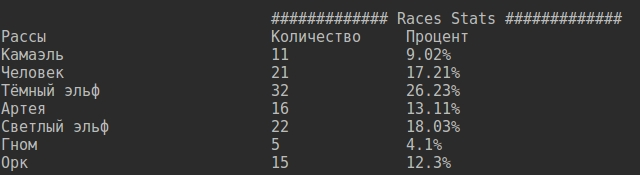
\includegraphics[scale=0.5]{4}
		\caption{- статистика по рассам} 
		\label{pic:pic_5} % название для ссылок внутри кода
	\end{center}
\end{figure}

\begin{figure}[H]
	\begin{center}
		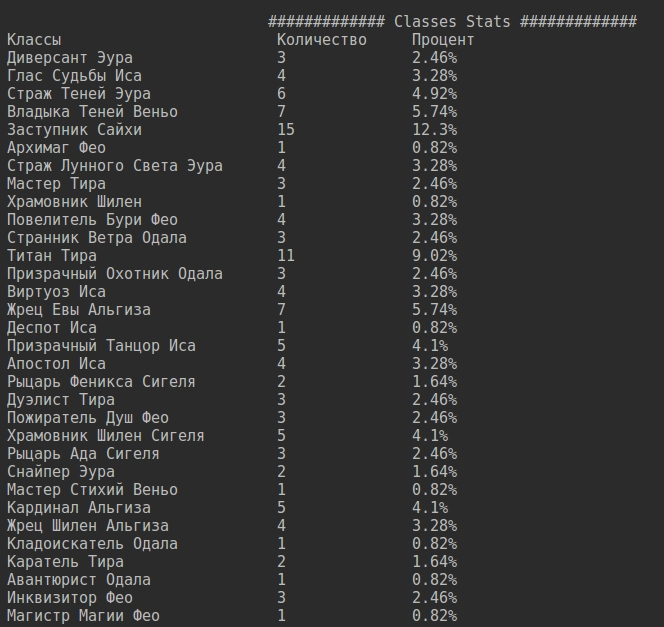
\includegraphics[scale=0.5]{5}
		\caption{- статистика по классам} 
		\label{pic:pic_6} % название для ссылок внутри кода
	\end{center}
\end{figure}

\begin{figure}[H]
	\begin{center}
		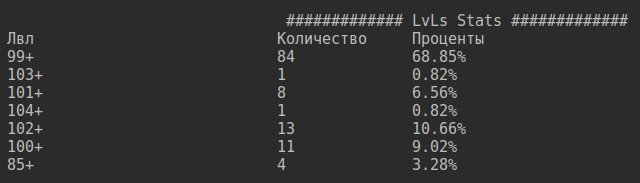
\includegraphics[scale=0.5]{6}
		\caption{- статистика по лвлу} 
		\label{pic:pic_7} % название для ссылок внутри кода
	\end{center}
\end{figure}

\begin{figure}[H]
	\begin{center}
		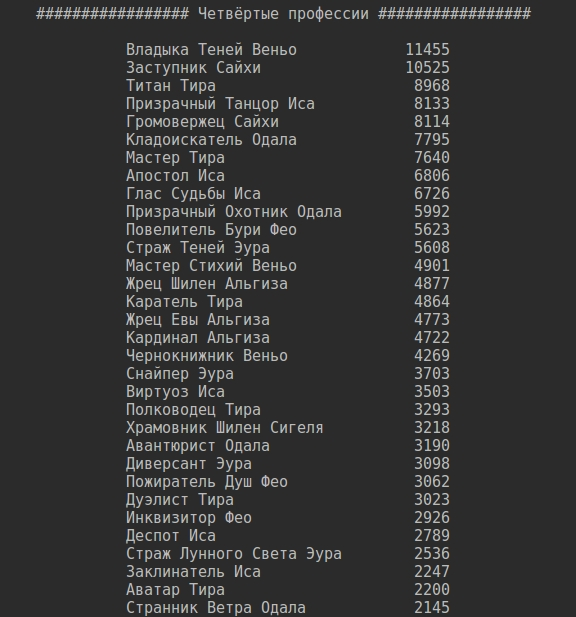
\includegraphics[scale=0.5]{7}
		\caption{- статистика по 4 профессиям} 
		\label{pic:pic_8} % название для ссылок внутри кода
	\end{center}
\end{figure}

\begin{figure}[H]
	\begin{center}
		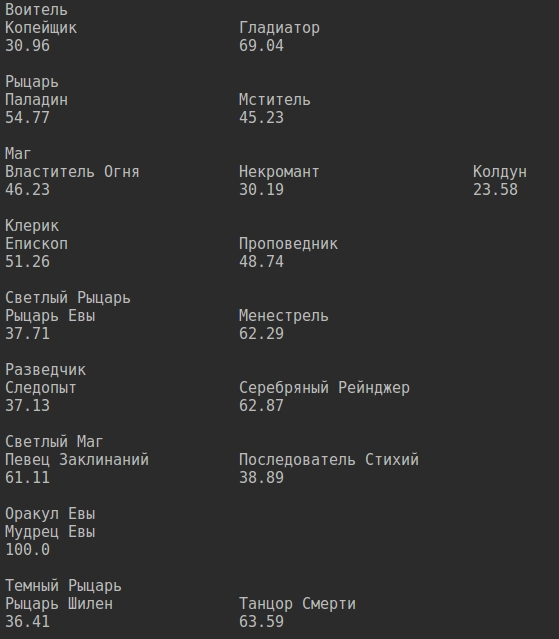
\includegraphics[scale=0.5]{8}
		\caption{- статистика по выбору профессий} 
		\label{pic:pic_9} % название для ссылок внутри кода
	\end{center}
\end{figure}

\begin{figure}[H]
	\begin{center}
		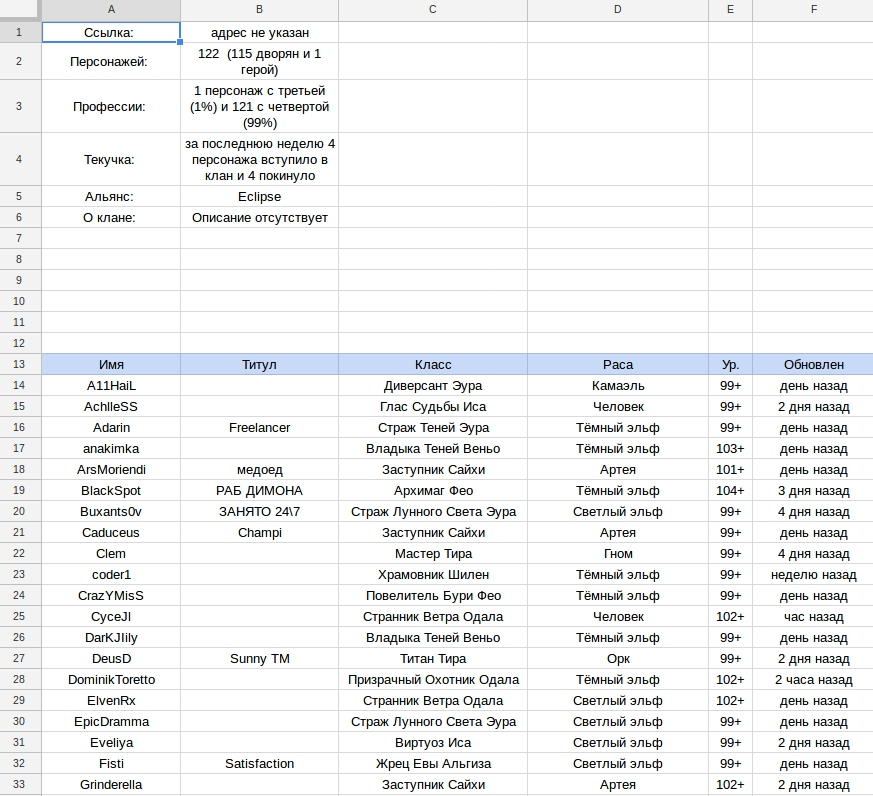
\includegraphics[scale=0.5]{9}
		\caption{- пример вывода данных в Google Doc} 
		\label{pic:pic_10} % название для ссылок внутри кода
	\end{center}
\end{figure}

\begin{figure}[H]
	\begin{center}
		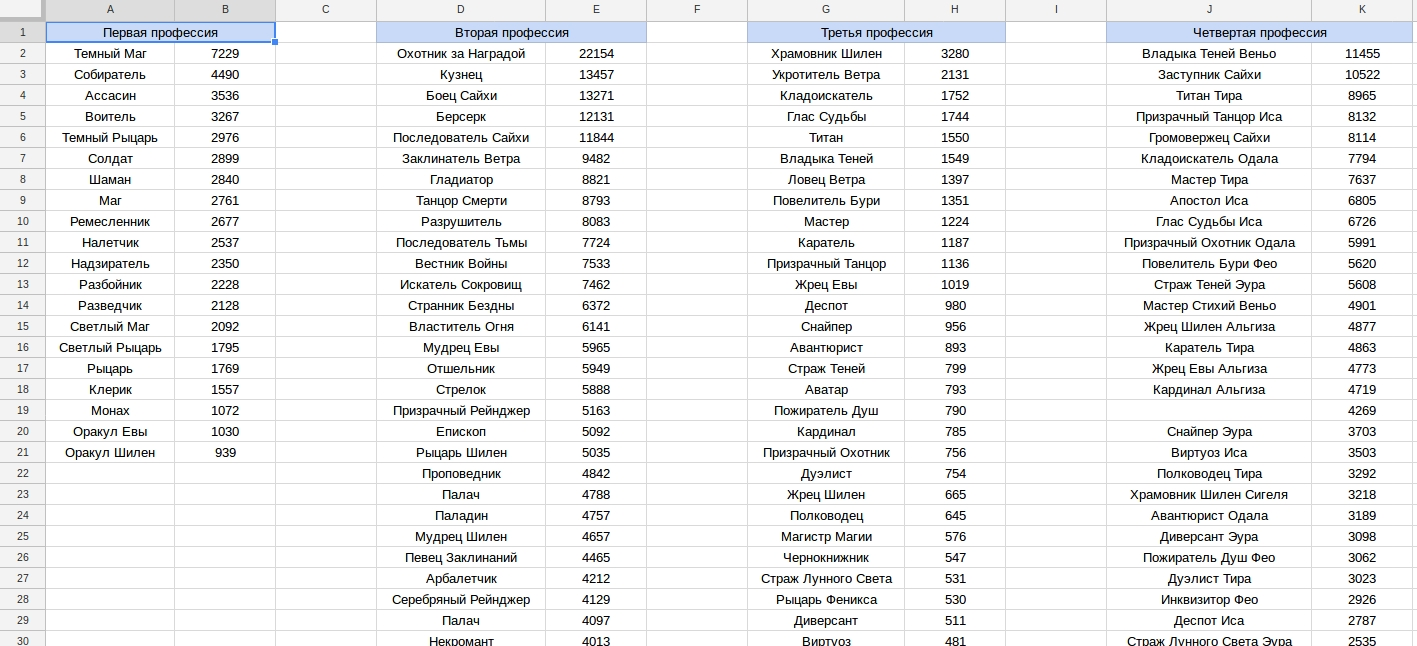
\includegraphics[scale=0.3]{10}
		\caption{- пример вывода данных в Google Doc} 
		\label{pic:pic_11} % название для ссылок внутри кода
	\end{center}
\end{figure}

\section{Вывод}
В данной лабораторной работе было получено большое количетво знаний в программировании на языке Python 3. Были освоены такие библиотеки, как BeautifulSoap4, urllib и gspread. Также все исхоные данные можно найти на репозитории:\\ https://github.com/Zenkin/l2onParsing.
\end{document}
